\documentclass{standalone}
\usepackage{tikz}
\usetikzlibrary{calc, shapes, patterns}

\begin{document}
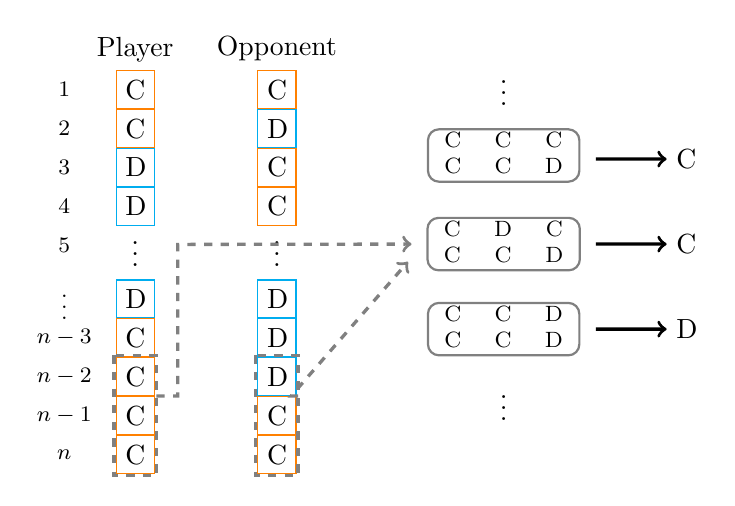
\begin{tikzpicture}[scale=.9]
    \tikzstyle{cooperator} = [rectangle, draw=orange, text width=.25cm]
    \tikzstyle{defector} = [rectangle, draw=cyan, text width=.25cm]


    % Histories ----------------------------------------
    \node (A) at (-.5, 0) {Player};
    \node (A1) at ($(A) + (0, -.57)$) [cooperator] {C};
    \node (A2) at ($(A1) + (0, -.55)$) [cooperator] {C};
    \node (A3) at ($(A2) + (0, -.55)$) [defector] {D};
    \node (A4) at ($(A3) + (0, -.55)$) [defector] {D};
    \node (A5) at ($(A4) + (0, -.55)$) {$\vdots$};
    \node (A6) at ($(A5) + (0, -.75)$) [defector] {D};
    \node (A7) at ($(A6) + (0, -.55)$) [cooperator] {C};
    \node (A8) at ($(A7) + (0, -.55)$) [cooperator] {C};
    \node (A9) at ($(A8) + (0, -.55)$) [cooperator] {C};
    \node (A10) at ($(A9) + (0, -.55)$) [cooperator] {C};

    \node (B) at ($(A) + (2, 0)$) {Opponent};
    \node (B1) at ($(B) + (0, -.57)$) [cooperator] {C};
    \node (B2) at ($(B1) + (0, -.55)$) [defector] {D};
    \node (B3) at ($(B2) + (0, -.55)$) [cooperator] {C};
    \node (B4) at ($(B3) + (0, -.55)$) [cooperator] {C};
    \node (B5) at ($(B4) + (0, -.55)$) {$\vdots$};
    \node (B6) at ($(B5) + (0, -.75)$) [defector] {D};
    \node (B7) at ($(B6) + (0, -.55)$) [defector] {D};
    \node (B8) at ($(B7) + (0, -.55)$) [defector] {D};
    \node (B9) at ($(B8) + (0, -.55)$) [cooperator] {C};
    \node (B10) at ($(B9) + (0, -.55)$) [cooperator] {C};

    \node (C) at ($(A) + (-1, 0)$) {};
    \node (C1) at ($(C) +  (0, -.57)$)  {\footnotesize{$1$}};
    \node (C2) at ($(C1) + (0, -.55)$) {\footnotesize{$2$}};
    \node (C3) at ($(C2) + (0, -.55)$) {\footnotesize{$3$}};
    \node (C4) at ($(C3) + (0, -.55)$) {\footnotesize{$4$}};
    \node (C5) at ($(C4) + (0, -.55)$) {\footnotesize{$5$}};
    \node (C6) at ($(C5) + (0, -.75)$) {\footnotesize{$\vdots$}};
    \node (C7) at ($(C6) + (0, -.55)$) {\footnotesize{$n - 3$}};
    \node (C8) at ($(C7) + (0, -.55)$) {\footnotesize{$n - 2$}};
    \node (C9) at ($(C8) + (0, -.55)$) {\footnotesize{$n -1$}};
    \node (C10) at ($(C9) + (0, -.55)$){\footnotesize{$n$}};
    % ---------------------------------------------------

    % Identifying inputs --------------------------------
    \draw[very thick, dashed, gray] ($(B8) + (-.3, .3)$)  rectangle ($(B10) + (.3, -.3)$);
    \draw[very thick, dashed, gray] ($(A8) + (-.3, .3)$)  rectangle ($(A10) + (.3, -.3)$);

    % % Strategy inputs
    \node (dummy) at ($(A) + (4.5, -2.75)$) {};
    \node (dummy_1) at ($(A) + (5.2, -.5)$) {$\vdots$};
    \node (dummy_2) at ($(A) + (5.2, -4.95)$) {$\vdots$};

    \node[draw=gray, inner sep=-.01mm, thick, rounded corners, font=\footnotesize] (action)  at (4.7, -2.75) {
        \begin{tabular}{ccc}
            C & D & C \\
            C & C & D \\
            \end{tabular}
    };
    \node[draw=gray, inner sep=-.01mm, thick, rounded corners, font=\footnotesize] (action_1)  at (4.7, -1.5) {
        \begin{tabular}{ccc}
            C & C & C \\
            C & C & D \\
            \end{tabular}
    };
    \node[draw=gray, inner sep=-.01mm, thick, rounded corners, font=\footnotesize] (action_2)  at (4.7, -3.95) {
        \begin{tabular}{ccc}
            C & C & D \\
            C & C & D \\
            \end{tabular}
    };

    \draw [very thick, gray, dashed, ->] ($(B8)!0.5!(B9) + (.3, 0)$) --
        ($(B8)!0.5!(B9) + (.2, 0)$) -- ($(dummy) + (-.65, -.25)$);
    \draw [very thick, gray, dashed, ->] ($(A8)!0.5!(A9) + (.3, 0)$) --
        ($(A8)!0.5!(A9) + (.6, 0)$) -- ($(A8)!0.5!(A9) + (.6, 2.14)$) --
        ($(dummy) + (-.6, 0)$);
    % Strategy outputs


    \node (output) at ($(dummy) + (3, 0)$) [right] {C};
    \node (output_1) at ($(dummy) + (3, -1.2)$) [right] {D};
    \node (output_2) at ($(dummy) + (3, 1.2)$) [right] {C};
    \draw [->, very thick] ($(dummy) + (2, 0)$) -- (output);
    \draw [->, very thick] ($(dummy) + (2, -1.2)$) -- (output_1);
    \draw [->, very thick] ($(dummy) + (2, 1.2)$) -- (output_2);
\end{tikzpicture}
\end{document}